\documentclass[12pt]{article}

\usepackage[a4paper, total={6in, 8in}]{geometry}

\usepackage{graphicx}
\graphicspath{ {./} }

\usepackage{hyperref}

\title{Homework 0}
\author{Stamate Valentin 2B4}

\begin{document}

\maketitle

  This documentation is about my result on finding the minimum value of any 
function. I used two methods: heuristic and deterministic. To have a known result
I used \textbf{Beale} function : \( f(x) = (1.5 - x_1 + x_1x_2)^2 + (2.25 - x_1 + x_1x_2^2)^2 + (2.625 - x_1 + x_1x_2^3)^2 \)
which has a minimum value of 0 in point \( X = (3, 0.5) \). The function can be easily modified by changing the fun() method, the number of components and the intervals.

\begin{center}
  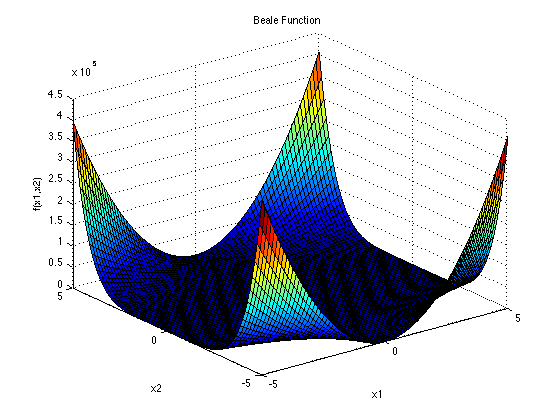
\includegraphics[scale=0.6]{beale.png}
\end{center}


  The algorithm will randomly choose a point X and calculate the function value in that point. To get a good result I'm gonna repeat the
process increasing the chance of getting the minimum point with a precision of 0.01. I will put the results in the next table.

\begin{center}
  \begin{tabular}{ c c c }
    & Deterministic & Heuristic \\ 
    Result & 0.656325 & 0.664847 \\  
   Point & \( (2.12, 7.689e^-6) \) & \( (2.16, 0.09) \) \\    
   Nr. Rep. & 1 & \( 1000 \) \\    
   Time(milis) & 14 & 3
  \end{tabular}
\end{center}

  As you can see, the result between deterministic approach and heuristic is pretty close. Even tho the deterministic algorithm
is the best, we got a greater time. More than that, the complexity of the deterministic algorithm is \( O( f(X) \prod_{i=1}^{n-1}m_i/\epsilon) \) where n is the dimension of X, \(m_i\) is the interval of every component of X, \(\epsilon\) is the precizion
and f(x) is the time for calculating the function. But heuristic algorithm has the time complexity of \( O(k n f(X)) \) where k is a constant and can be ignored. So the heuristic function wins even if it's not the exact result but the time complexity is much better than the deterministic algorithm.

\section*{Biblograpy}

\begin{enumerate}
  \item \url{http://www-optima.amp.i.kyoto-u.ac.jp/member/student/hedar/Hedar_files/TestGO_files/Page288.htm}
  \item \url{https://www.sfu.ca/~ssurjano/beale.html#:~:text=The%20Beale%20function%20is%20multimodal,corners%20of%20the%20input%20domain.}
  \item \url{https://diego.assencio.com/?index=6890b8c50169ef45b74db135063c227c}
  \item \url{https://stackoverflow.com/questions/19555121/how-to-get-current-timestamp-in-milliseconds-since-1970-just-the-way-java-gets}
  \item \url{https://www.youtube.com/watch?v=VnwjxityDLQ&ab_channel=CodeBullet}
  \item \url{https://www.youtube.com/watch?v=9zfeTw-uFCw&list=PLRqwX-V7Uu6bJM3VgzjNV5YxVxUwzALHV&ab_channel=TheCodingTrain}
\end{enumerate}


\end{document}